\documentclass{article} % For LaTeX2e
\usepackage{nips13submit_e,times}
\usepackage{hyperref}
\usepackage{url}
\usepackage{amsmath}
\usepackage{amssymb}
\usepackage{amsthm}
%\documentstyle[nips13submit_09,times,art10]{article} % For LaTeX 2.09
\usepackage[utf8]{inputenc}
\raggedbottom

\title{An importance sampling procedure\\ for estimating crop yield}


\author{
J. Benjamin Cook\\
\texttt{jbenjamincook@gmail.com}
}

% The \author macro works with any number of authors. There are two commands
% used to separate the names and addresses of multiple authors: \And and \AND.
%
% Using \And between authors leaves it to \LaTeX{} to determine where to break
% the lines. Using \AND forces a linebreak at that point. So, if \LaTeX{}
% puts 3 of 4 authors names on the first line, and the last on the second
% line, try using \AND instead of \And before the third author name.

\newcommand{\fix}{\marginpar{FIX}}
\newcommand{\new}{\marginpar{NEW}}
\usepackage{graphicx}
\usepackage{float}
\usepackage{caption}

\nipsfinalcopy % Uncomment for camera-ready version

\begin{document}


\maketitle

% \begin{abstract}
% The abstract paragraph should be indented 1/2~inch (3~picas) on both left and
% right-hand margins. Use 10~point type, with a vertical spacing of 11~points.
% The word \textbf{Abstract} must be centered, bold, and in point size 12. Two
% line spaces precede the abstract. The abstract must be limited to one
% paragraph.
% \end{abstract}

\section{Introduction}

Unprecedented amounts of data are available on modern farms. From yield monitors to weather sensors to infrared imaging, farmers are able to keep track of every detail on their farms. However, most farmers are not taking advantage of this data. Much of the data is never reviewed after being collected. The data that is reviewed remains inaccessible, trapped in complicated legacy software, agronomist reports, and countless pages of spreadsheets.

Agricultural production lags far behind other industries in using data to make decisions, but data-based decision-making will be essential in the future. Farming is a challenging business. Reduced availability of water and increasing input costs are squeezing farmers’ bottom lines during a time of extreme volatility in the commodities markets. New regulations on irrigation, pesticide use, and fertilizer application mean farmers must find a new way to boost yield. Soon, using data to optimize decision-making will no longer be a novel luxury – it will be essential for farmers to stay in business.

The purpose of this project is to develop and assess a stochastic procedure for estimating crop yield in a maize field with an eye toward making in-season forecasts. Giving farmers insight about how much yield to expect in their fields will arm them to effectively compete against professional traders in the futures market.

\section{Background}

Consider a corn field $\Omega$ and a yield function $f(x)$ that returns bushels per acre at any location in the field $x$. Total yield, in bushels can be evaluated by multiplying the area of the field, $|\Omega|$, by the integral, $I = \int_{\Omega} f(x) dx$. Assuming we can evaluate the function $f$ at any location in the field, we can estimate the integral with $\hat{I}_{mc} = \frac{1}{N} \sum_i f(x_i)$, where the $x_i$ are drawn uniformly from the area $\Omega$. However, since yield is not distributed evenly throughout the field, this ``vanilla'' Monte Carlo approach results in unnecessarily high variance. Instead, it is possible to draw samples from a (possibly unnormalized) proposal distribution that is somehow ``close'' to $f$ and then correct for the fact that the samples are no longer uniform. With importance sampling, the integral is estimated as:
$$\hat{I}_{is} = \int f(x) dx = \int g(x) \frac{f(x)}{g(x)}dx \approx \frac{1}{N}\sum_{x_i \sim g(.)} \frac{f(x_i)}{g(x_i)}$$
This approach assumes that $f(x)$ and $g(x)$ are normalized probability densities. Alternatively, we can use unnormalized functions if we correct for them as follows:
$$\hat{I}_{is} = \sum_i w_i f(x_i)$$
where $w_i = \frac{\widetilde{w}_i}{\sum_i \widetilde{w}_i}$ and $\widetilde{w}_i = \frac{f(x_i)}{g(x_i)}$ \cite{murphy}.

In order to build a procedure that is robust and effective, this paper addresses the following questions:
\begin{enumerate}
\item After the first pass, how should one derive an importance sampling function?
\item What is the best method for drawing samples from the importance sampling function?
\item On the second pass, how many points do we need to sample to achieve an acceptably low level of variance?
\end{enumerate}

\section{Data}

The data come from a corn field in Butler County, Nebraska that was planted and harvested in 2009. Measurements are logged by a grain yield monitor which is connected to sensors on the arms of the tractor as it harvests the corn. The yield monitor records an estimate of yield in bushels per acre and geolocation approximately six times per second. The full dataset contains $16,898$ points. Figure \ref{fig:raw} displays the raw data as a yield map in the left panel and a histogram of yield in the right panel.

\begin{figure}
\begin{center}
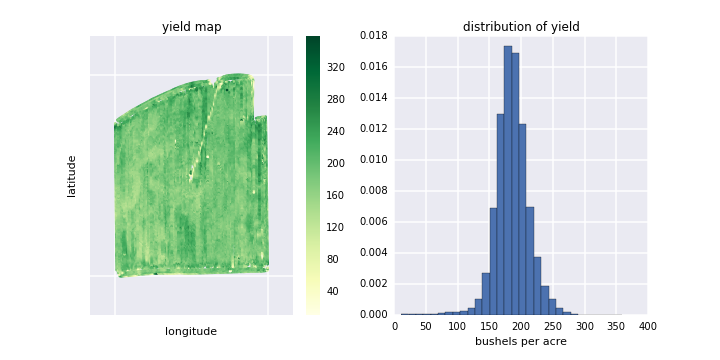
\includegraphics[width=0.8\textwidth]{figures/raw_data}
\caption{A yield map with the raw data and the distribution of yield at all measured locations}%
\label{fig:raw}
\end{center}
\end{figure}

Although the data coverage for this field is extensive, the sampling methods require that we can evaluate a yield function $f(.)$ at any continuous point $x_i \in \Omega$. Because of this requirement, $f(x_i)$ is defined as the average of the five nearest neighbors to point $i$. This is essnetially a pre-processing step and does not have a major impact on final results.

Because total number of bushels in the field is the quantity of interest, but data are in units of bushels per acre, we need an estimate of the total number of acres in the field. One convenient way to estimate the area is to do rejection sampling: draw points from a rectangle of known area and multiply the area of the rectangle by the fraction of points drawn that fall within the field boundary. Using this approach, the number of acres is found to be approximately 63.7. Figure \ref{fig:mcarea} shows Monte Carlo samples where locations inside the field, $\Omega$, are blue.

\begin{figure}
\begin{center}
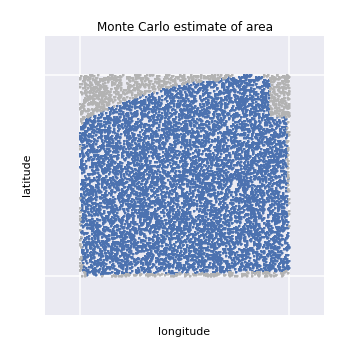
\includegraphics[width=0.4\textwidth]{figures/mc_area}
\caption{Monte Carlo estimate of field area}%
\label{fig:mcarea}
\end{center}
\end{figure}


% One difficulty in analyzing these data is that the points are dense and irregularly spaced. At times during harvest, the tractor drove over the same spot more than once, so two points in almost the same location have very different estimates of yield. In order to compensate for this problem, a k-Nearest Neighbors regressor is fit to the data as a pre-processing step. This allows the recovery of a 100 $\times$ 100 point grid with a somewhat stronger signal. Points outside of the polygon of observed data are dropped. For the most part, this pre-processing step does not seriously affect the yield map or the distribution of yield. The two differences are now we no longer have overlapping points in the yield map and we have fewer outliers in the distribution.

% \begin{figure}[H]
% \begin{center}
% 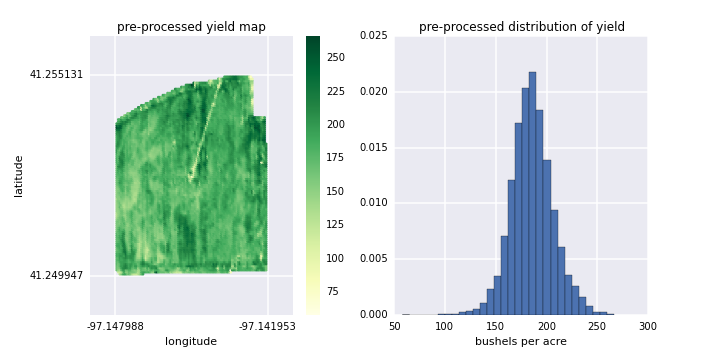
\includegraphics[width=0.8\textwidth]{figures/preprocessed_data}
% \caption{A yield map with the pre-processed data and the distribution of yield at all measured locations}%
% \label{fig:preprocessed}
% \end{center}
% \end{figure}

\section{Method}

The importance sampling procedure for estimating yield consists of four steps:
\begin{enumerate}
\item Collect a small number of samples from $f(.)$
\item Construct the proposal function $g(.)$
\item Sample from $g(.)$
\item Use the samples to estimate yield
\end{enumerate}
This section enumerates each of the four steps.

The first step is to collect $N_1$ yield samples from the field. This is constrained to be a small number because it corresponds to someone actually walking the field and collecting stalks at $N_1$ randomly selected locations throughout the field.

Currently there is a strong simplifying assumption here: we can evaluate the actual yield function at these locations. That is, we can use the $N_1$ corn stalks to evaluate yield in bushels per acre at the sampled locations. In reality, inferring yield in bushels per acre based on volume of the grain from these $N_1$ stalks or based on height and circumference of the stalks will require a separate step.

% \begin{figure}[H]
% \begin{center}
% 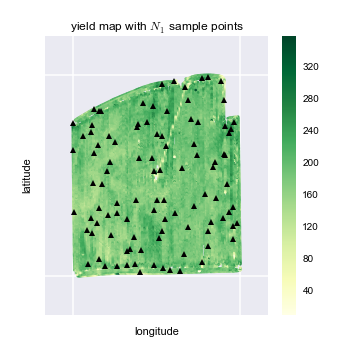
\includegraphics[width=0.4\textwidth]{figures/sampled_points}
% \caption{100 randomly selected points throughout the field}%
% \label{fig:sampled}
% \end{center}
% \end{figure}

The next step is to define the proposal function $g(.)$. Here, it is important to use a function that is somehow close to the true yield function so samples are concentrated in high yield areas. One simple way to build a function that is close to the true yield function is to fit a Gaussian Process (GP) to the $N_1$ samples. A GP is a distribution over functions and, assuming the mean is set to zero, is fully specified by a covariance kernel, $K(x_i, x_j)$ \cite{rasmussen}. One common form for the covariance function is a squared exponential: $$\sigma^2 \exp{\left(-\|x_i - x_j\|^2 / \phi\right)}$$ Assuming we know the hyper-parameters, $\sigma^2$ and $\phi$, we now have a function that we can use for importance sampling: $$g(x_{new}) = K(x_{new}, X)K^{-1}(X,X)y$$ which corresponds to the mean of the GP. Here, $X$ is the vecotor of locations for the $N_1$ samples and $x_{new}$ is the location of any arbitrary new point. In theory, the hyper-parameters $\sigma^2$ and $\phi$ should not matter since we do not actually need a perfect model for the $N_1$ samples from the first pass. In practice, the GP is only ``close'' to the yield function for a relatively small range of the hyper-parameter values. Figure \ref{fig:gpfit} shows $g(x)$ for $x \in \Omega$.

\begin{figure}
\begin{center}
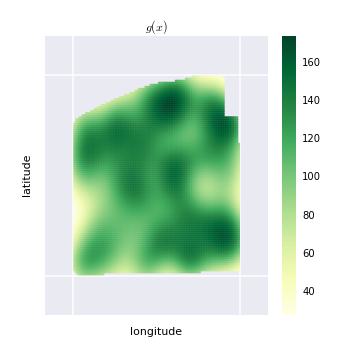
\includegraphics[width=0.4\textwidth]{figures/gp}
\caption{A Gaussian Process fit to the first $N_1$ points}%
\label{fig:gpfit}
\end{center}
\end{figure}

% This addresses the first question being considered in this paper. A GP fit to the first $N_1$ samples is a reasonable method for finding a proposal function. Other possibilities include kernel density estimates and Gaussian mixture models. If yield is relatively unimodal, a simple multivariate Gaussian would suffice as a proposal function.

The third step is to draw samples from $g(x)$ to find good candidate points for evaluating crop yield. Two Markov Chain Monte Carlo algorithms were used to sample from $g(x)$: Slice Sampling \cite{neal} and Metropolis-Hastings \cite{chib}. The M-H algorithm is preferred in this case because it does a good job of sampling from $g(x)$ and is faster than Slice Sampling. The proposal for the M-H samples is $q(x^{*}|x) \sim \mathcal{N}(x, \gamma)$, where $\gamma$ is set to 0.002. 100 burn-in samples are discarded and thinning parameter is set to three, so that every third sample is saved. Points drawn outside of $\Omega$ are defined to be $-\infty$ and are therefore never accepted. The M-H algorithm performs well because even though $g(x)$ is multi-modal, the modes are relatively flat. Figure \ref{fig:mh} shows 1,000 M-H samples from $g(x)$ and Figure \ref{fig:trace} shows trace plots for longitude and latitude.

\begin{figure}
\begin{center}
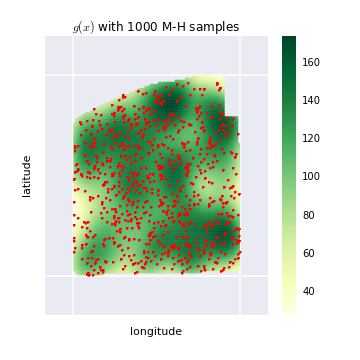
\includegraphics[width=0.4\textwidth]{figures/gp_samples}
\caption{Samples drawn from the importance sampling function}%
\label{fig:mh}
\end{center}
\end{figure}

\begin{figure}
\begin{center}
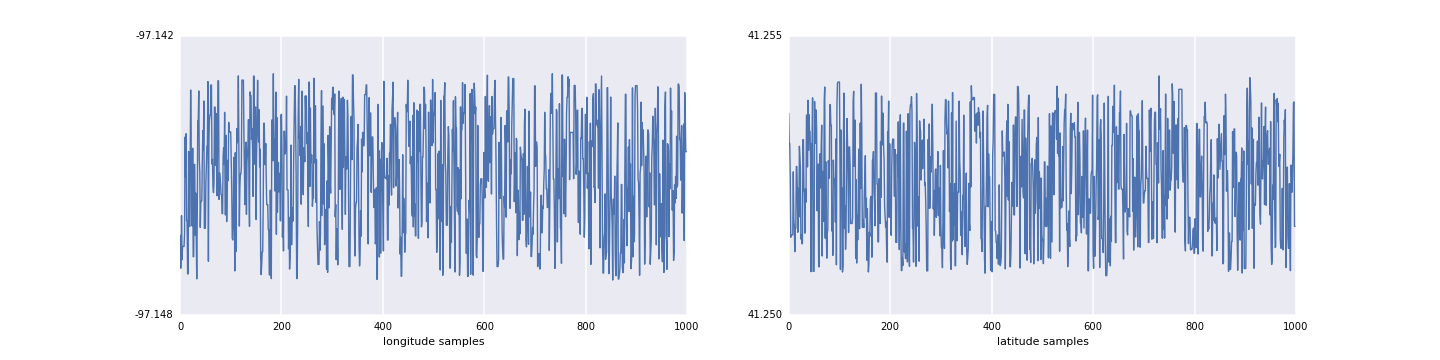
\includegraphics[width=0.8\textwidth]{figures/trace}
\caption{Trace plots of longitude and latitude samples from the M-H algorithm}%
\label{fig:trace}
\end{center}
\end{figure}

\section{Results}

The importance sampling procedure is an effective way to estimate the number of bushels the field yields. Unsurprisingly, as the number of M-H draws increases, the the variance of the estimate decreases. Table \ref{tab:results} show the average estimate and the standard deviation of those estimates for $N_{mc} = 100, 500$, and $1,000$. Each experiment was performed 100 times. The left panel of Figure \ref{fig:results} shows histograms of the three levels of M-H draws and the right panel shows a box plot of the estimates and variance.

\begin{table}[H]
\begin{center}
\caption{Results}%
\begin{tabular}{rcr}
\hline
% {Model} & {parameters}  &  \shortstack{effective \\ parameters} &     $R^2$ &     RMSE \\
$N_{mc}$ & Bushels &  $\textrm{sd}(\hat{I}_{is})$ \\
\hline
100   & 11,987 & 160 \\
500   & 11,979 & 79 \\
1,000 & 11,988 & 58\\
\hline
\end{tabular}
\label{tab:results}
\end{center}
\end{table}

\begin{figure}
\begin{center}
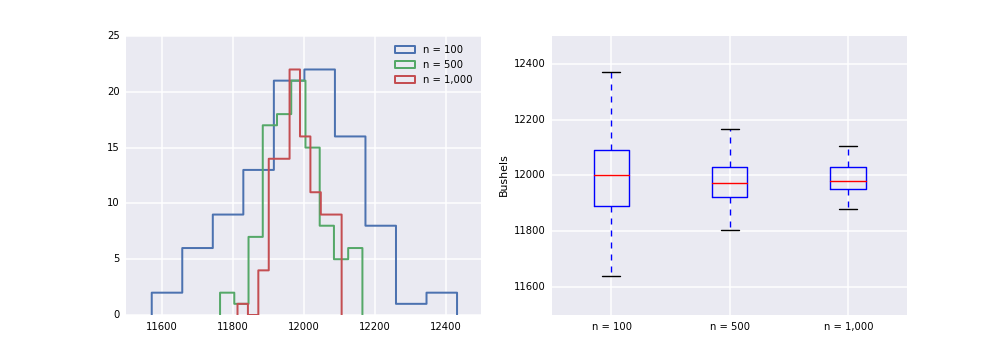
\includegraphics[width=0.8\textwidth]{figures/results}
\caption{Distribution of estimates of $|\Omega|\hat{I}_{is}$ and variance of estimate as the number of Metropolis samples increases}%
\label{fig:results}
\end{center}
\end{figure}

In practice, how many M-H samples need to be drawn would have to be determined by the farmers and agronomists who use this procedure. Samples are relatively expensive in the sense that each one needs to be collected by hand. Fortunately, even with only $N_{mc}= 100$ samples, the standard deviation of 160 is less than 2 \% of the number of bushels. This low variance makes the importance sampling method practical for estimating yield in real situations.

\section{Conclusion}
Stochastic optimization provides an important set of tools for estimating the crop yield in irregularly shaped fields. Fitting a GP to a few samples and then drawing several more importance samples from this proposal function decreases variance of estimated crop yield. This procedure can be used in a prediction setting with one additional step: by modeling how physical characteristics of the plant throughout the growing season drive yield at harvest.

\bibliographystyle{acm}
\bibliography{sample}

\end{document}





